\documentclass[11pt, oneside]{article}   	% use "amsart" instead of "article" for AMSLaTeX format
\usepackage[margin=1in]{geometry}               % See geometry.pdf to learn the layout options. There are lots.
\geometry{letterpaper}                   	% ... or a4paper or a5paper or ... 
%\geometry{landscape}                		% Activate for rotated page geometry
%\usepackage[parfill]{parskip}    		% Activate to begin paragraphs with an empty line rather than an indent
\usepackage{graphicx}				% Use pdf, png, jpg, or eps§ with pdflatex; use eps in DVI mode
						% TeX will automatically convert eps --> pdf in pdflatex		
\usepackage{amssymb}
\usepackage{amsmath}
\usepackage{indentfirst}
\usepackage{enumitem}
\usepackage{mathptmx}
\usepackage{float}

%SetFonts

%SetFonts

\setcounter{secnumdepth}{3} % default value for 'report' class is "2"

\title{APPM 4560 Laboratory 1 Report}
\author{Rhys Olsen\\
\texttt{rhys.olsen@colorado.edu}
 \and Jessica Petty\\
 \texttt{jessica.petty@colorado.edu}
 }
\date{September 26, 2016}

\begin{document}
\maketitle
\section{Simulating Random Permutations}
\subsection{Simulating One Random Permutation}

Given the size-increasing ordered list of the finite set consisting of natural numbers $\left\{1, \dots, \right\}$ for some $n \in \mathbb{N}$, the following algorithm will simulate a random permutation of the list:

%Algorithm to Generate Random Permutation 

\subsubsection{Algorithm to Generate Random Permutation}\label{sssec:perm}
\begin{enumerate}[leftmargin=30pt,labelindent=65pt,itemindent=30pt]
\item[\textsc{step 1:}] Simulate and store $n$ random variables $U_1, \dots, U_n \sim \text{Uniform}(0,1)$

\item[\textsc{step 2:}] Define some $f$ that maps each $\text{Uniform}\left(0,1 \right)$ random variable to the index at which it was created

\item[\textsc{step 3:}] Order the $\text{Uniform}\left(0,1 \right)$ random variables in decreasing order

\item[\textsc{step 4:}] Apply $f$ to each $U_i$ to produce the permutation of integers
\end{enumerate}

\subsubsection{Probability of Observing a Fixed Permutation}
Fixing a particular permutation $\sigma = (f(1), \dots, f(n))$ of the ordered list $\left\{1, \dots, n\right\}$, for a given random permutation generated according to~\ref{sssec:perm}, since the first number in the permutation is equally likely to be any of $\left\{1, \dots, n\right\}$, The probability that the first number in the permutation is $f(1)$, which is the first number in $\sigma$, is $n$. In general, having already fixed the first $i$ numbers in a permutation to match the first $i$ of $\sigma$, the equal likelihood of any remaining number being next in the permutation implies that the probability the $i + 1$th number in the permutation will match the $i + 1$th of $\sigma$ is $\frac{1}{n - i}$. Conditioning on each successive number of the permutation matching $\sigma$ means that the probability of a randomly generated permutation matching $\sigma$ is:
\begin{equation}\label{eqn:fix}
  p_{\text{fixed}} = \frac{1}{n} \times \frac{1}{n - 1} \times \dots \times \frac{1}{1} = \frac{1}{n!}
\end{equation}

\subsection{\textit{X}: Number of Random Observations of a Particular Permutation}\label{ssec:x}
We define the random variable $X$ to be the number of random permutations of $\left\{1, \dots, n\right\}$ that equal $\sigma$ among $m$ such permutations generated by~\ref{sssec:perm}. Observe that the $m$ randomly generated permutations are independent. Since each permutation matches $\sigma$ with probability $p_{\text{fixed}} = \frac{1}{n!}$, we can treat $X$ as the number of successes among $m$ independent trials where a given success occurs with probability $p_{\text{fixed}}$. Under this treatment, the random variable $X$ therefore has a \textit{binomial} distribution with trial count $m$ and success probability $p_{\text{fixed}} = \frac{1}{n!}$. For the simulation of $X$ discussed in following sections, we are experimentally interested in the values $m = 6000$ and $n = 7$.

Now, given that \textit{X} has a \textit{binomial} distribution, we seek its probability mass function $f_S(x)$ expectation $\mathbb{E}[X]$.

To generalize, for $B \sim \text{Binomial}(n, p)$, of which $X$ is a particular case, we seek $f_B(k) = P(B = k)$. Note that for there to be exactly $k$ consecutive successes among $n$ trials each of which succeeds with probability $p$, the remaining $k - n$ trials must have been failures. By the independence of the trials, this event occurs with probability $p^k(1-p)^{n-k}$. Finally, note that there are ${n \choose k}$ distinct ways of permuting these trials, each of which amounts to exactly $k$ successes among the $n$ trials. Therefore $f_B(k) = {b \choose k}p^k(1-p)^{n-k}, 0 \leq k \leq n$.

Additionally, We know that $\mathbb{E}[B] = np$, which we can prove using the definition of expected value:

\begin{equation*}
\begin{split}
  \mathbb{E}[B] = \sum_{k=0}^{n}kP(B=k)=
  \sum_{k=0}^{n}k\binom{n}{k}p^k(1-p)^{n-k}=\\
  \sum_{k=0}^{n}k \frac{n!}{k!(n-k)!}p^k(1-p)^{n-k}=
  \sum_{k=1}^{n}\frac{n!}{(k-1)!(n-k)!}p^k(1-p)^{n-k}
\end{split}
\end{equation*}
because we can remove the term corresponding to $k=0$. If we now introduce two new variables, \textit{j} and \textit{m} such that $j=k-1$ and $m=n-1$ then we have:

$$\mathbb{E}[B]=\sum_{j=0}^{m}\frac{(m+1)!}{j!(m-j)!}p^{j+1}(1-p)^{m-j}=(m+1)p\sum_{j=0}^m\frac{m!}{j!(m-j)!}p^j(1-p)^{m-j}$$\\
Now, remembering the Binomial Theorem:
\begin{equation}
  (a+b)^m=\sum_{y=0}^{m}\frac{m!}{y!(m-y)!}a^yb^{m-y}
  \label{eqn:bt}
\end{equation}
we get the following result when we let $a=p$ and $b=1-p$:\\
\begin{equation*}
  \sum_{j=0}^{m}\frac{m!}{y!(m-y)!}p^j(1-p)^{m-j}=
  \sum_{y=0}^{m}\frac{m!}{y!(m-y)!}a^yb^{m-y}=
  (a+b)^m=(p-(1-p))^m=1^m=1
\end{equation*}\\
and therefore we can conclude that:
$$\mathbb{E}[B]=(m+1)p\cdot 1=np$$

Noting that $X \sim \text{Binomial}(m,\frac{1}{n!})$, $\mathbb{E}[X] = \frac{m}{n!}$. For the constants $m = 6000$ and $n = 7$, this is $\mathbb{E}[X] = \frac{6000}{7!} = \frac{6000}{5040} = \frac{25}{21} \sim 1.19$.

\subsection{\textit{Y}: Number of Random Permutations Needed To Match A Particular Permutation}
We define the random variable $Y$ to be the number of random permutations of $\left\{1, \dots, n\right\}$ generated by~\ref{sssec:perm} needed to witness $\sigma$ once among the permutations. As was the case in \ref{ssec:x}, $Y$ can be described in terms of independent trials each succeeding with probability $p_{\text{fixed}} = \frac{1}{n!}$. In contrast to the random varaible $X$, however, the random variable $Y$ represents the number of independent trials that succeed with probability $p_{\text{fixed}}$ needed for the last trial to be a success. Under this characterization, $Y$ is a \textit{geometric} random variable with success probability $p_{\text{fixed}}$. We seek its probability mass function $f_Y(y)$ and expectation $\mathbb{E}[Y]$. For the simulation of $Y$ mentioned in sections to follow, we are experimentally interested in the value of $n = 7$.

For $k$ to be the first instance in a series of independent trials for a success with probability $p$, all of the previous $k - 1$ trials must have failed with probability $(1 - p)$. By the independence of the trials, a geometric random variable $G \sim \text{Geometric}(p)$ has probability density function $f_G(k) = p(1-p)^{k-1}, 1 \leq k \leq \infty$. Since $Y \sim \text{Geometric}(\frac{1}{n!})$, $f_Y(y) = \frac{1}{n!} * (1 - \frac{1}{n!})^{y-1}, 1 \leq k \leq \infty$. For $n = 7$, this is $f_Y(y) = \frac{1}{7!} * (1 - \frac{1}{7!})^{y-1} = \frac{1}{5040} * (1 - \frac{1}{5040})^{y-1}, 1 \leq k \leq \infty$.

The expectation of $G$ is given by the equation:
\begin{equation*}
\begin{split}
\mathbb{E}[G] =
\sum_{k = 1}^{\infty}k p_G(k) =
\sum_{k = 1}^{\infty}k p(1-p)^{k-1} =\\
p \sum_{k = 1}^{\infty}k (1 - p)^{k-1} =
p \frac{\partial}{\partial p} \left[-\sum_{k = 1}^{\infty}(1 - p)^k\right]
\end{split}
\end{equation*}

Because $(1-p)^{0} = 1$, we can rewrite the sum under the differential operator to produce:
\begin{equation*}
\mathbb{E}[G] = p \frac{\partial}{\partial p} \left[1 - \sum_{k = 0}^{\infty}(1 - p)^k\right]
\end{equation*}

Recall the formula for the geometric series:
\begin{equation}
\sum_{k = 0}^{\infty}a^n = \frac{1}{1-a}
\label{eqn:gs}
\end{equation}

We can rewrite $\mathbb{E}[G]$ using equation~\ref{eqn:gs} as:
\begin{equation*}
p \frac{\partial}{\partial p} \left[1 - \frac{1}{1 - (1 - p)}\right] =
p \frac{\partial}{\partial p} \left[1 - \frac{1}{p}\right] =
p \left(\frac{1}{p^2}\right) =
\frac{1}{p}
\end{equation*}

Therefore $\mathbb{E}[G] = \frac{1}{p}$, and as a consequence, we have $\mathbb{E}[Y] = \frac{1}{1/n!} = n!$, where again $n$ gives the upper bound on the set $\{1, \dots, n\}$ being permuted. For $n = 7$, this is $\mathbb{E}[Y] = 7! = 5040$.

\subsection{Comparison of Theoretical Distribution of \textit{X} With Simulation}

\begin{figure}[H]
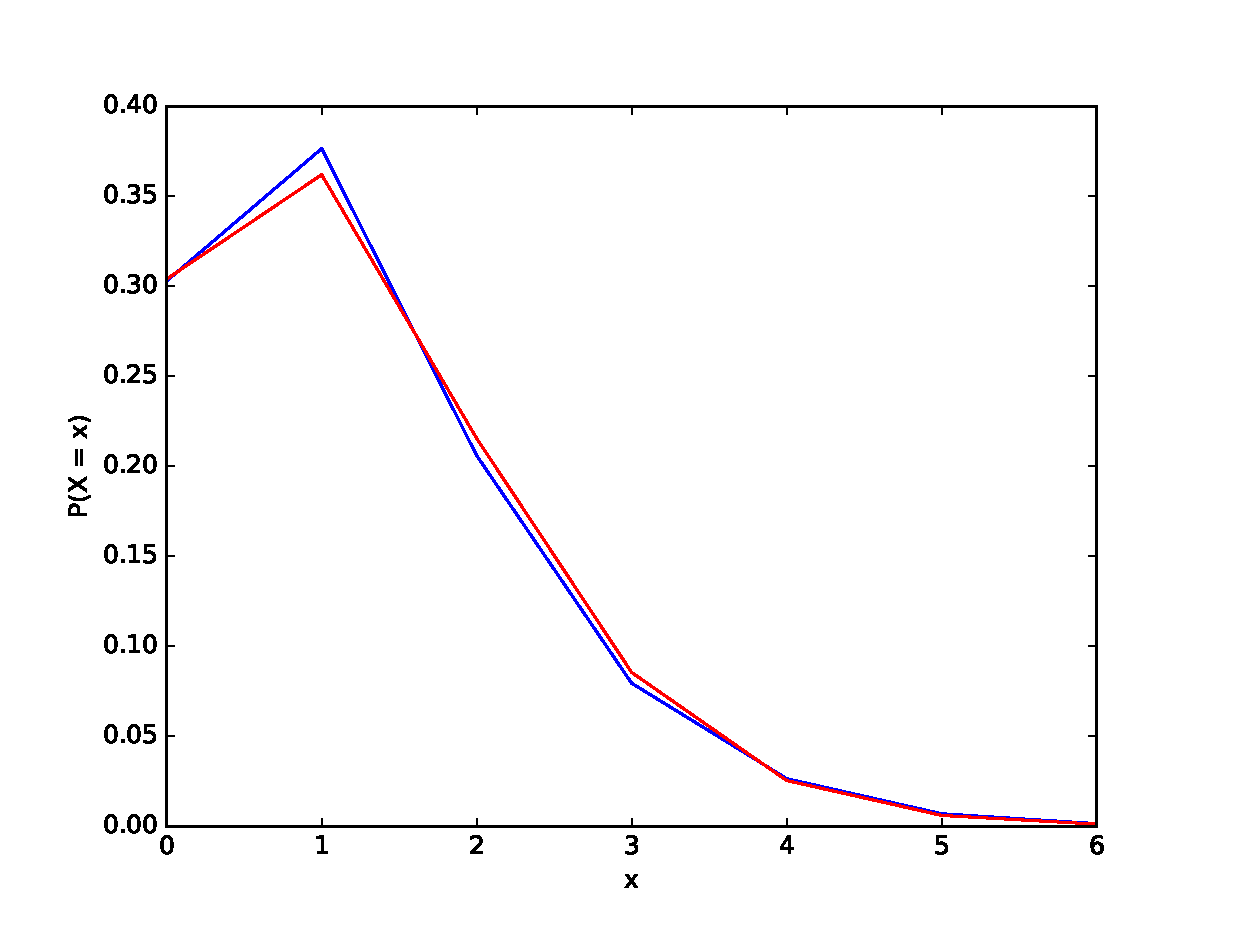
\includegraphics[scale=.5]{part_1_problem_4}
\caption{Plot of likelihood versus support value of the random variable $X$ with $m = 6000$ and $n = 7$ for $k = 2000$ computer simulations of the random variable (in blue) compared with the theoretical distribution that $X$ respects (in red). Note that the computer simulations have been normalized such that the sum of the histogram bins is $1$. Notice that the experimental plot is quite similar to the theoretical one, with slightly less variance.}
\label{fig:x}
\end{figure}

We implement a procedure to simulate $X$ with $m = 6000$ and $n = 7$ by generating $m$ permutations using the algorithm given in \ref{sssec:perm} and counting the number of those $m$ permutations that equal $\sigma = (6, 7, 2, 5, 1, 4, 3)$. Using this procedure, We simulate $X$ $k = 2000$ times and plot its histogram against the theoretical distribution for $X$ in figure~\ref{fig:x}. Our plot shows strong agreement between the theoretical distribution and its simulation, suggesting that both the analysis of the random variable $X$ and the implementation of the simulation are correct.

\subsection{Comparison of Theoretical Distribution of \textit{Y} With Simulation}

\begin{figure}[H]
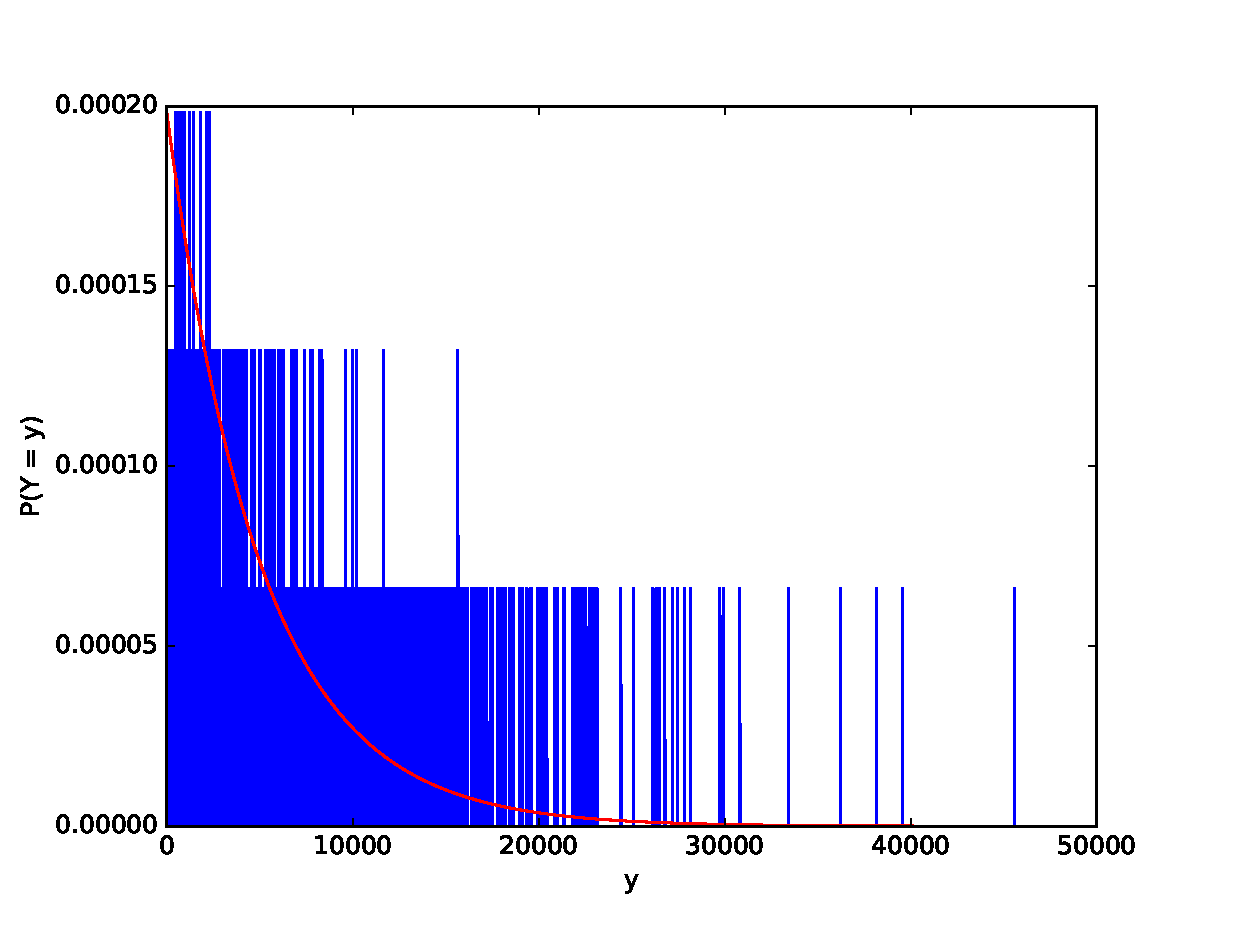
\includegraphics[scale=.5]{part_1_problem_5}
\caption{Plot of likelihood versus support value of the random variable $Y$ with $n = 7$ for $k = 2000$ computer simulations of the random variable (in blue) compared with the theoretical distribution that $X$ respects (in red). Note that the computer simulations have been normalized such that the tallest of the histogram bins is equal in height to the mode value of the geometric model, which is at $Y = 1$. While it's less obvious than in figure~\ref{fig:x} that the simulations agree with the theoretical model due to how simulating $Y$ $k = 2000$ times samples the larger support more sparsely and results in very low counts of each measured event, the density of the blue lines in any given horizontal region and simulation sample count threshold agrees with the proportion of blue in the same horizontal region and sample count threshold that is below the red line representing the probability density function.}
\label{fig:y}
\end{figure}

We implement a procedure to simulate $Y$ with $n = 7$ by generating permutations using the algorithm given in \ref{sssec:perm}, keeping a count of how many random permutations we generate, and returning this count as soon as a permutation is generated that equals $\sigma = (6, 7, 2, 5, 1, 4, 3)$. Using this procedure, We simulate $Y$ $k = 2000$ times and plot its histogram against the theoretical distribution for $Y$ in figure~\ref{fig:y}. Once again, our plot shows strong agreement between the theoretical distribution and its simulation, inspiring confidence in the correctness of our analysis and simulation.

\section{Computing Performance of Retrieving Algorithms}
\subsection{}
[Brief definition of $Q_A$ here.] We seek $\mathbb{E}[Q_A]$.

$Q_A$'s probability mass function $f_{Q_A}(x)$ represents the probability of position $x$ being the location of the number 1. Note that each possible position of the number 1 is equally likely with probability $1 / n$, so $f_{Q_A}(x) = 1 / n, 1 \leq x \leq n$. This means $\mathbb{E}[Q_A] = \sum_{k=1}^{n} \frac{1}{n} k = \frac{1}{n} \sum_{k = 1}^{n} k = \frac{1}{n} \frac{n (n + 1)}{2} = \frac{n + 1}{2}$.
\subsection{}
\subsection{}
\subsection{}
Blah blah blah binary search trees blah blah blah $\in O(\log_2(n))$. Can we find specific constants?
\subsection{}

\end{document}
